\section{Numerical comparison of the \texorpdfstring{$\kl$}{kl} and split-\texorpdfstring{$\kl$}{kl} inequalities (30 points) [Yevgeny]}

We consider a ternary random variable $X$ taking values $X \in \Bigl\{0,\tfrac12,1\Bigr\}$.
Let
\[
  p_{0}= \P \bigl(X=0\bigr), \qquad
  p_{\frac12}= \P\bigl(X=\tfrac12\bigr), \qquad
  p_{1}= \P \bigl(X=1\bigr).
\]
and set \(p_{0}=p_{1}=(1-p_{\frac12})/2\), so that the probabilities of \(X=0\) and \(X=1\) are equal, and there is only one parameter \(p_{\frac12}\), which controls the 
probability mass of the central value.
\\[2mm]
We now want to compare the two bounds $\kl$ and split-$\kl$ as a function of \(p_{\frac12}\in[0,1]\). The upper $\kl$ bound for \(p-\hat p_{n}\) is given by
\[
\klui\Bigl(\hat p_{n},
        \tfrac{\ln\frac{n+1}{\delta}}{n}
  \Bigr)
  -\hat p_{n}
\]
and the split-$\mathrm{kl}$ bound is
\begin{equation} \label{eq:split-kl-bounds}
   b_{0}+\sum_{j=1}^{K} \Bigg(  \alpha_{j}\,
   k_{1}^{-1,+}\!\Bigl(\hat{p}_{\mid j},
                       \frac{1}{n}\ln\!\frac{K}{\delta}\Bigr) - \hat{p}_{\mid j} \Bigg),
\end{equation}
where $\hat{p}_{\mid j}= \frac{1}{n}\sum_{i=1}^{n}X_{i\mid j}$ and $X_{i\mid j}= \1[X_{i}\ge b_{j}]$ denotes the elements of the binary decomposition of $X_{i}$.
\\[2mm]
For this experiment, we find that the domain is $b_0=0, b_1 = 0.5, b_2=1$ and the $K=2$ segments are $\alpha_1=\alpha_2=1/2$. So eq. \ref{eq:split-kl-bounds} simplifies to:
\[
\tfrac{1}{2} \Big( \klui(\hat{p}_{\mid 1}, \epsilon ) - \hat{p}_{\mid 1} \Big)
+ \tfrac{1}{2}\Big( \klui(\hat{p}_{ \mid2}, \epsilon ) - \hat{p}_{\mid 2} \Big),   
\]
where $\epsilon = \tfrac{1}{n} \ln \tfrac{K}{\delta}  = \tfrac{1}{n} \ln \tfrac{2}{\delta}.$
In figure \ref{fig:splitkl} we see a plot of $\kl$ and split-$\kl$.

\begin{figure}[ht]
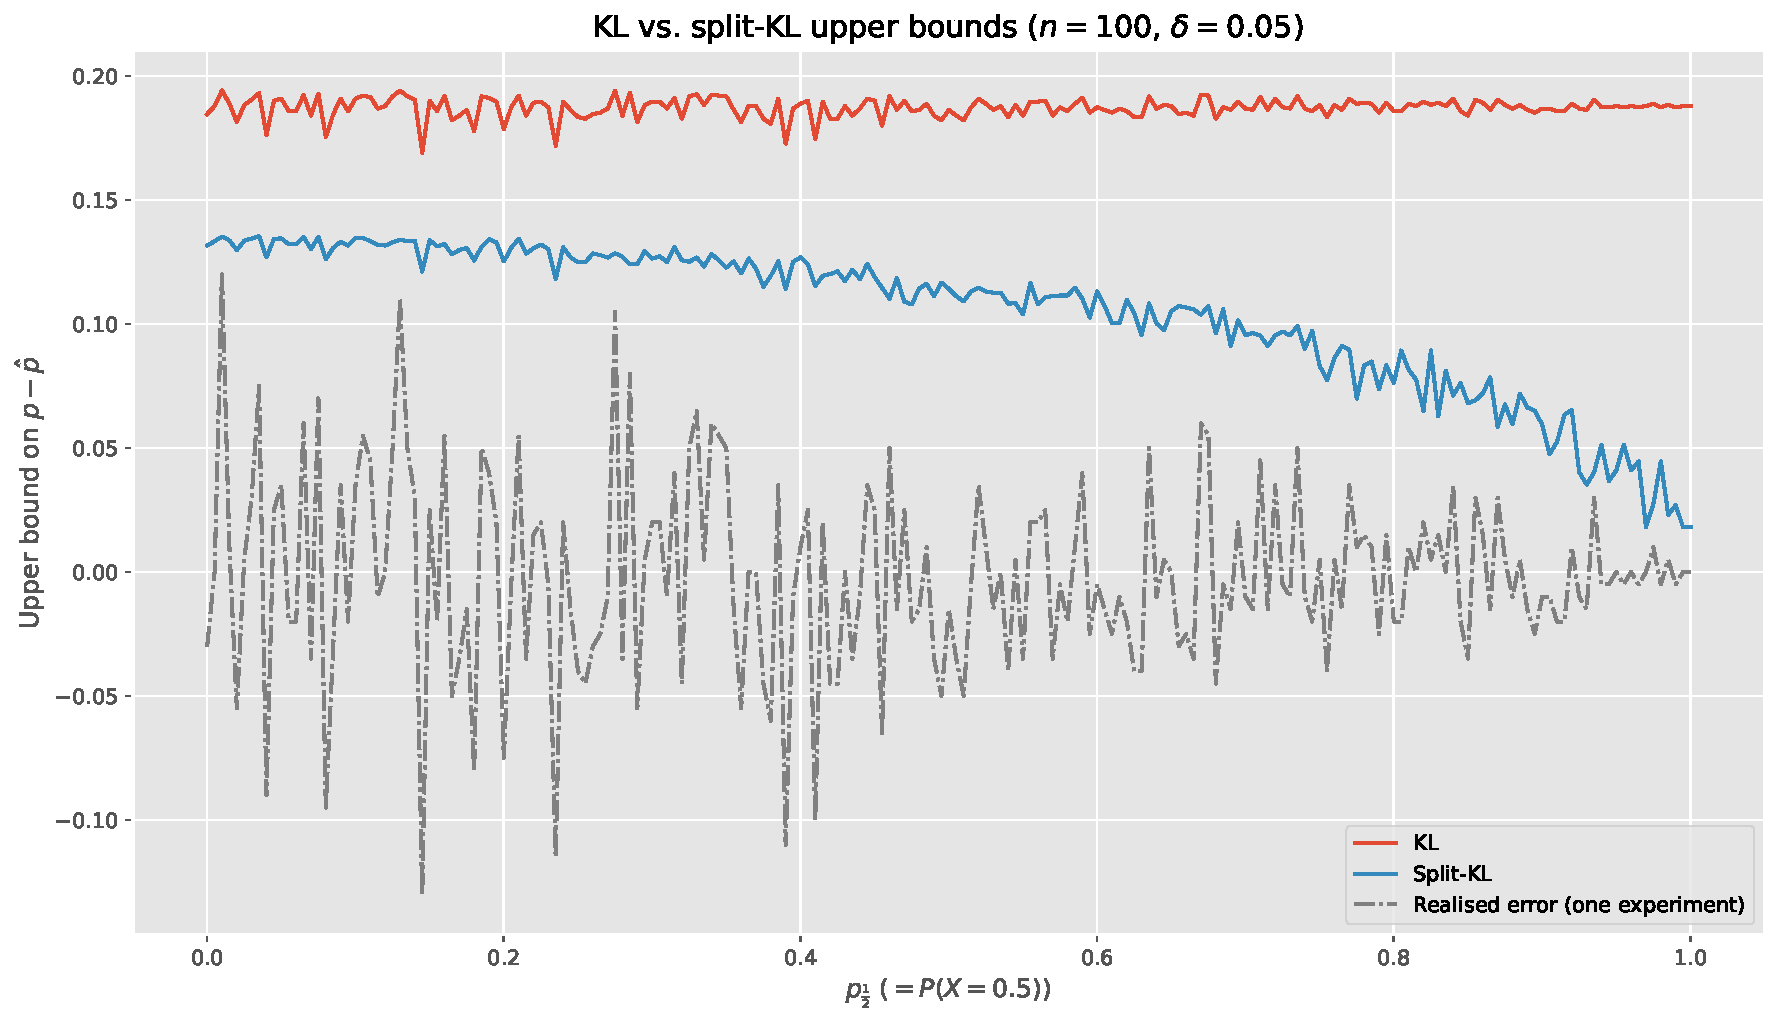
\includegraphics[scale=0.5]{figures/splitkl_vs_kl.pdf}
\label{fig:splitkl}
\end{figure}


\subsection*{Brief discussion}
Because the true mean is fixed at 0.5 for every choice of $p_{1/2}$, the empirical mean
fluctuates around $0.5$, with variance depending on the distribution’s
shape. 

The dashed curve is the realized error in the single sample that was
drawn for each $p_{1/2}$

Let us consider what happens when $p_{\frac{1}{2}} \rightarrow 1$. In that case most of 
the probability mass is pushed to the center value 0.5, and the two outcomes (0 and 1) become very rare since their probabilities $p0 = p1 = (1-p_{\frac{1}{2}})/2 \rightarrow  0$.
Consequently the variance of X given by $\Var(X)=0.25(1 -p_{\frac{1}{2}}) \rightarrow  0$.
Hence the empirical mean is in practice locked very tightly
around the true mean 0.5 once $p_{\frac{1}{2}}$ get closer to 1.
\\[2mm]
Split-$\kl$ decomposes $X$ into the two binary indicators:
$$
X_{\mid 1} = \1[X \geq 0.5], \quad X_{\mid 2} = \1[X \geq 1].
$$
Their expectations are
\begin{align*}
    p_{\mid 1} &= \P(X \geq 0.5) = 1 - p_0  \rightarrow 1, \\
    p_{\mid 2} &= \P(X \geq 1.0) = p_1      \rightarrow 0
\end{align*}
as $p_{\frac{1}{2}} \rightarrow 1$.
\\[2mm]
When a Bernoulli parameter is very close to 1 or 0, the
$\kl$-inverse difference $\klui(\hat{p},\epsilon)-\hat{p}$ is proportional to $\hat{p}(1-\hat{p})$ and therefore goes to zero.
\\[2mm]
For the split-$\kl$ bound these two tiny differences are multiplied by
$\alpha_1 = \alpha_2 = 0.5$ and then added, so the whole bound collapses
toward 0 as soon as $X$ almost never takes the extreme values.
That is why in figure \ref{fig:splitkl} observe split-$\kl$ close to 0 for $p_{\frac{1}{2}}$ close to 1.
